\documentclass[10pt,a4paper,oneside]{article}
\usepackage[utf8]{inputenc}
\usepackage{amsmath}
\usepackage{amsfonts}
\usepackage{amssymb}
\usepackage{graphicx}
\usepackage{breqn}
\usepackage{tikz} % system block diagram
\usepackage{textcomp}
\usetikzlibrary{shapes,arrows} % system block diagram
\usepackage{booktabs}
\usepackage[framed,numbered,autolinebreaks,useliterate]{mcode} % matlab code block
\author{Yangang Cao}
\date{February 13, 2019}
\newcommand{\degree}{^\circ}
\tikzset{
	delay/.style    = {draw, thick, rectangle, minimum height = 3em,
		minimum width = 3em},
	sum/.style      = {draw, circle, node distance = 2cm}, 
	prod/.style     = {draw, circle, node distance = 2cm},
	input/.style    = {coordinate}, % Input
	output/.style  = {coordinate} % Output
}
% Defining string as labels of certain blocks.
\newcommand{\product}{$\displaystyle \times$}
\newcommand{\delay}{\large$z^{-1}$}
\begin{document}

\title{First-Order Low/Highpass Filter Design}
\maketitle 

The signal can be seen as a set of partials having different frenquencies and amplitudes. The filter can modify the amplitude of partials according to their frenquency.

\section{Definition of Low/Highpass Filters}

The two types of filters can be defined according to the following classification:

\begin{itemize}
	\item {\bfseries Lowpass (LP)} filters select low frenquencies up to the cut-off frenquency $f_c$ and attenuate frenquencies higher than $f_c$. Additionally, a resonance may amply frenquencies around $f_c$.
	\item {\bfseries Highpass (HP)} filters select high frenquencies higher than $f_c$ and attenuate frenquencies below $f_c$, possibly with a resonance around $f_c$.
\end{itemize}

The lowpass with resonance is very often used in computer music to simulate an acoustical resonating structure; the highpass filter can remove undesired very low frequencies.

\section{Canonical Form}
There are various ways to implement a filter, the simplest being the canonical filter, as shown in following figure for a second-order filter, which can be implemented by the defference equations
\[
x_h(n) = x(n) - a_1x_h(n-1) - a_2x_h(n-2)
\]
\[
y(n) = b_0x_h(n) + b_1x_h(n-1) + b_2x_h(n-2),
\]



\begin{center}
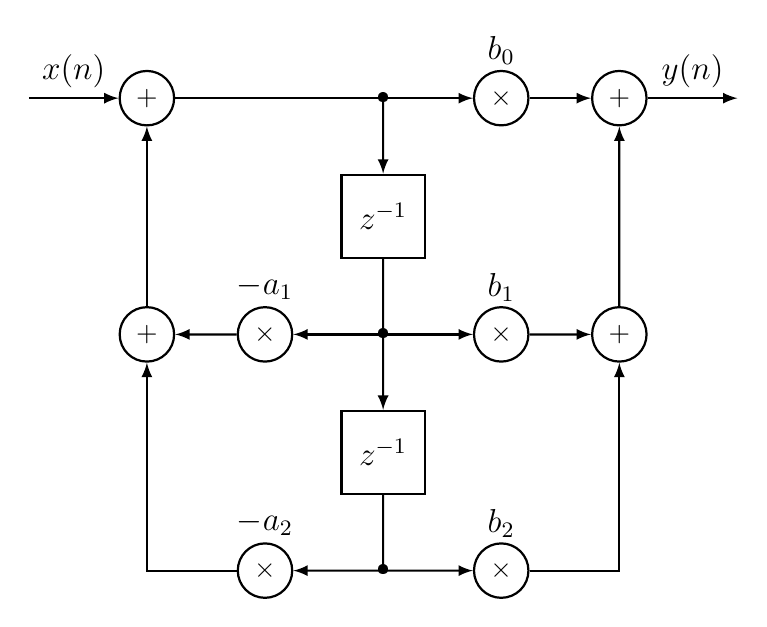
\begin{tikzpicture}[auto, thick, node distance=0.6cm, >=latex, scale = 0.75]
\draw
% Drawing the blocks of first filter 
node at (0,0)[sum] (s1) {$+$}
node at (6,0)[prod] (p1) {\product} node[above of = p1] {\large$b_0$}
node at (8,0)[sum] (s2) {$+$}
node at (4,-2) [delay] (d1) {\delay}
node at (0,-4) [sum] (s3) {$+$}
node at (2,-4) [prod] (p2) {\product} node[above of = p2] {\large$-a_1$}
node at (6,-4) [prod] (p3) {\product} node[above of = p3] {\large$b_1$}
node at (8,-4) [sum] (s4) {$+$}
node at (4,-6) [delay] (d2) {\delay}
node at (2,-8) [prod] (p4) {\product} node[above of = p4] {\large$-a_2$}
node at (6,-8) [prod] (p5) {\product} node[above of = p5] {\large$b_2$};

\draw[->](-2,0) -- node {\large$x(n)$}(s1);
\draw[->](s1) -- node {} (p1);
\draw[->](p1) -- node {} (s2);
\draw[->](s2) -- node {\large$y(n)$} (10,0);
\draw[->](4,0) -- node {} (d1);
\draw[->](d1) -- node {} (d2);
\draw[<->](p2) -- node {} (p3);
\draw[->](p2) -- node {} (s3);
\draw[->](s3) -- node {} (s1);
\draw[->](p3) -- node {} (s4);
\draw[->](s4) -- node {} (s2);
\draw[-](d2) -- node {} (4,-8);
\draw[<->](p4) -- node {} (p5);
\draw[->](p4) -| node {} (s3);
\draw[->](p5) -| node {} (s4);

\draw
node at (4,0) {\textbullet} 
node at (4,-4){\textbullet}
node at (4,-8){\textbullet};
\end{tikzpicture}
\end{center}
and leads to the transfer function by setting $a_2 = b_2 = 0$, this reduces to a first-order filter which, can be used to implement an allpass, lowpass or highpass with the coefficients of following table
\begin{center}
	\begin{tabular}{cccc}
	\toprule  %添加表格头部粗线
	 & {$b_0$}&{$b_1$}&{$a_1$}\\
	\midrule  %添加表格中横线
	Lowpass&K/(K+1)& K/(K+1) & (K-1)/(K+1)\\
	Highpass& 1/(K+1)& -1/(K+1) & (K-1)/(K+1)\\
	Allpass&(K-1)/(K+1)&1&(K-1)/(K+1)\\
	\bottomrule %添加表格底部粗线
	\end{tabular}
\end{center}
where $K$ depends on the cut-off frequency $f_c$ by
\[
K=\tan(\pi f_c/f_S).
\]

\section{First-Order Allpass-Based Filter}

In this section we introduce a special class of parametric filter structures for lowpass, highpass, bandpass and bandreject filter functions. These filter structures are easily tunable by changing only one or two coefficients. They play an important role for real-time control with minimum computational complexity.

The basis for parametric first- and second-order IIR filters is the first- and second-order allpass filter. We will first discuss the first-order allpass and show simple lowpass and highpass filters, which consist of a tunable allpass filter together with a direct path.

A first-order allpass filter is given by the transfer function
\[
A(z) = \frac{z^{-1} + c}{1 + cz^{-1}}
\]
\[
c = \frac{\tan(\pi f_c/f_S) - 1}{\tan(\pi f_c/f_S) + 1},
\]
and the corresponding difference equations
\[
x_h(n) = x(n) - cx_h(n-1)
\]
\[
y(n) = cx_h(n) + x_h(n-1),
\]
which can be realized by the following block diagram,

\begin{center}
	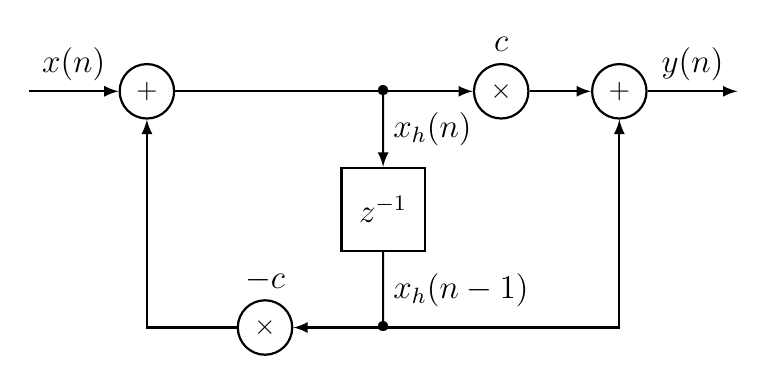
\begin{tikzpicture}[auto, thick, node distance=0.6cm, >=latex, scale = 0.75]
	\draw
	% Drawing the blocks of first filter 
	node at (0,0)[sum] (s1) {$+$}
	node at (6,0)[prod] (p1) {\product} node[above of = p1] {\large$c$}
	node at (8,0)[sum] (s2) {$+$}
	node at (4,-2) [delay] (d1) {\delay}
	node at (2,-4) [prod] (p2) {\product} node[above of = p2] {\large$-c$};
	
	\draw[->](-2,0) -- node {\large$x(n)$}(s1);
	\draw[->](s1) -- node {} (p1);
	\draw[->](p1) -- node {} (s2);
	\draw[->](s2) -- node {\large$y(n)$} (10,0);
	\draw[->](4,0) -- node {\large$x_h(n)$} (d1);
	\draw[->](p2) -| node {} (s1);
	\draw[-](d1) -- node {\large$x_h(n-1)$} (4,-4);
	\draw[<->](p2) -| node {} (s2);
	
	\draw
	node at (4,0) {\textbullet} 
	node at (4,-4){\textbullet};
	
	\end{tikzpicture}
\end{center}
and corresponding state and output equations are:
\[
x_h(n) = -cx_h(n-1) +x(n)
\]
\[
y(n) = (1-c^2)x_h(n-1) + cx(n).
\]

Actually, the state and output equations represent the same meaning as the difference equations, but difference in format. The difference equations are usually easy to comprehend, howere, state and output equations are more widely used in modern control theory, so we implement all kinds of filters by this format. The first-order allpass filter implementation can be obtained by the following {\bfseries Matlab} code.
\begin{lstlisting}
function y = firstallpass(audio, para)
% y = firstallpass(audio, para)
% Author: Yangang Cao
% Applies a allpass filter to the input signal.
% para is the normalized cut-off frequency in (0,1)
c = (tan(pi*para/2)-1) / (tan(pi*para/2)+1);
x = 0;
x_1 = 0;
for n = 1:length(audio)
	x_1 = -c * x + audio(n);
	y(n) = (1 - c^2) * x + c * audio(n);
	x = x_1;
end
\end{lstlisting}

\section{First-Order Low/Highpass Filter}
A first-order lowpass/highpass filter can be achieved by adding or subtracting (+/--) the output signal from the input signal of a first-order allpass filter.The transfer function of a lowpass/highpass filter is then given by

\[
H(z) = \frac{1}{2}(1 \pm A(z))\quad(LP/HP+/-)
\]
\[
A(z) = \frac{z^{-1} + c}{1 + cz^{-1}}
\]
\[
c = \frac{\tan(\pi f_c/f_S) - 1}{\tan(\pi f_c/f_S) + 1}.
\]

where a tunable first-order allpass $A(z)$ with tuning parameter $c$ is used. The plus sign (+) denotes the lowpass operation and the minus sign (--) the highpass operation. The block diagram in following figure represents the operations involved in performing the low/highpass filtering.
\begin{center}
	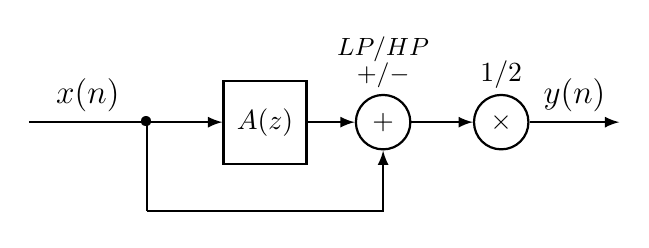
\begin{tikzpicture}[auto, thick, node distance=0.6cm, >=latex, scale = 0.75]
	\draw
	node at (2,0)[delay] (d1) {$A(z)$}
	node at (4,0)[sum] (s1) {$+$} 
	node[above of = s1]{\small$+/-$} node[above of=s1,above=1]{\small{$LP/HP$}}
	node at (6,0) [prod] (p1) {\product} node[above of = p1]{$1/2$};
	
	\draw[-](-2,0) -- node {\large$x(n)$}(0,0);
	\draw[->](0,0) -- node {} (d1);
	\draw[->](d1) -- node {} (s1);
	\draw[->](s1) -- node {} (p1);
	\draw[->](p1) -- node {\large$y(n)$} (8,0);
	\draw[-](0,0) -- node {} (0,-1.5);
	\draw[->](0,-1.5) -| node {} (s1);
	
	\draw
	node at (0,0) {\textbullet};
	
	\end{tikzpicture}
\end{center}

The difference equations of first-order lowpass filter are:
\[
x_h(n) = x(n) - cx_h(n-1)
\]
\[
y(n) = \frac{1+c}{2}x_h(n) + \frac{1+c}{2}x_h(n-1),
\]
and corresponding state and output equations are:
\[
x_h(n) = -cx_h(n-1) +x(n)
\]
\[
y(n) = \frac{1-c^2}{2}x_h(n-1) + \frac{1+c}{2}x(n).
\]
A first-order lowpass filter implementation can be obtained by the following {\bfseries Matlab} code.
\begin{lstlisting}
function y = aplowpass(audio, para)
% y = aplowpass(audio, para)
% Author: Yangang Cao
% Applies a lowpass filter to the input signal.
% para is the normalized cut-off frequency in (0,1)
c = (tan(pi*para/2)-1) / (tan(pi*para/2)+1);
x = 0;
x_1 = 0;
for n = 1:length(audio)
	x_1 = -c * x + audio(n);
	y(n) = ((1-c^2)/2) * x + (1+c)/2 * audio(n);
	x = x_1;   
end
\end{lstlisting}

The difference equations of first-order highpass filter are: 
\[
x_h(n) = x(n) - cx_h(n-1)
\]
\[
y(n) = \frac{1-c}{2}x_h(n) + \frac{c-1}{2}x_h(n-1),
\]
and corresponding state and output equations are:
\[
x_h(n) = -cx_h(n-1) +x(n)
\]
\[
y(n) = \frac{c^2-1}{2}x_h(n-1) + \frac{1-c}{2}x(n).
\]
A first-order highpass filter implementation can be obtained by the following {\bfseries Matlab} code.
\begin{lstlisting}
function y = aphighpass(audio, para)
% y = aphighpass(audio, para)
% Author: Yangang Cao
% Applies a highpass filter to the input signal.
% para is the normalized cut-off frequency in (0,1)
c = (tan(pi*para/2)-1) / (tan(pi*para/2)+1);
x = 0;
x_1 = 0;
for n = 1:length(audio)
	x_1 = -c * x + audio(n);
	y(n) = ((c^2-1)/2) * x + (1-c)/2 * audio(n);
	x = x_1;  
end
\end{lstlisting}
\end{document}
